\documentclass[11pt,a4paper,oneside]{article}

\title{\textbf{Route2Dam: Provide information on day trips to Rotterdam for students at Utrecht University}\newline \newline \newline}
\date{\today}
\author{Sorin Dragan, Evangelia Giannikou, \\Mikhail Ternyuk, Olusanmi Hundogan}
% \pagenumbering{gobble}
\pagenumbering{arabic}

\usepackage{eurosym}
\usepackage{hyperref}
\usepackage{subfig}
\usepackage{amsmath}
\usepackage{amssymb}
\usepackage{tabularx,booktabs}
\usepackage{multicol}
\usepackage{array}
\usepackage{float}
\usepackage[english]{babel}
\usepackage{quoting}
\usepackage{csquotes}
\usepackage{enumitem}
\usepackage{natbib}
\usepackage{xcolor}
\usepackage{subfiles}
\usepackage{ragged2e}
\usepackage{lmodern,textcomp}
\usepackage{graphicx}
\usepackage{subcaption}
\usepackage{titling}
\newcolumntype{M}[1]{>{\centering\arraybackslash}m{#1}}
\usepackage[backend=biber, sorting=none]{biblatex}
\usepackage[total={6.5in, 10in}]{geometry}
\addbibresource{references.bib}

\begin{document}

\maketitle
% \begin{figure}[H]
%     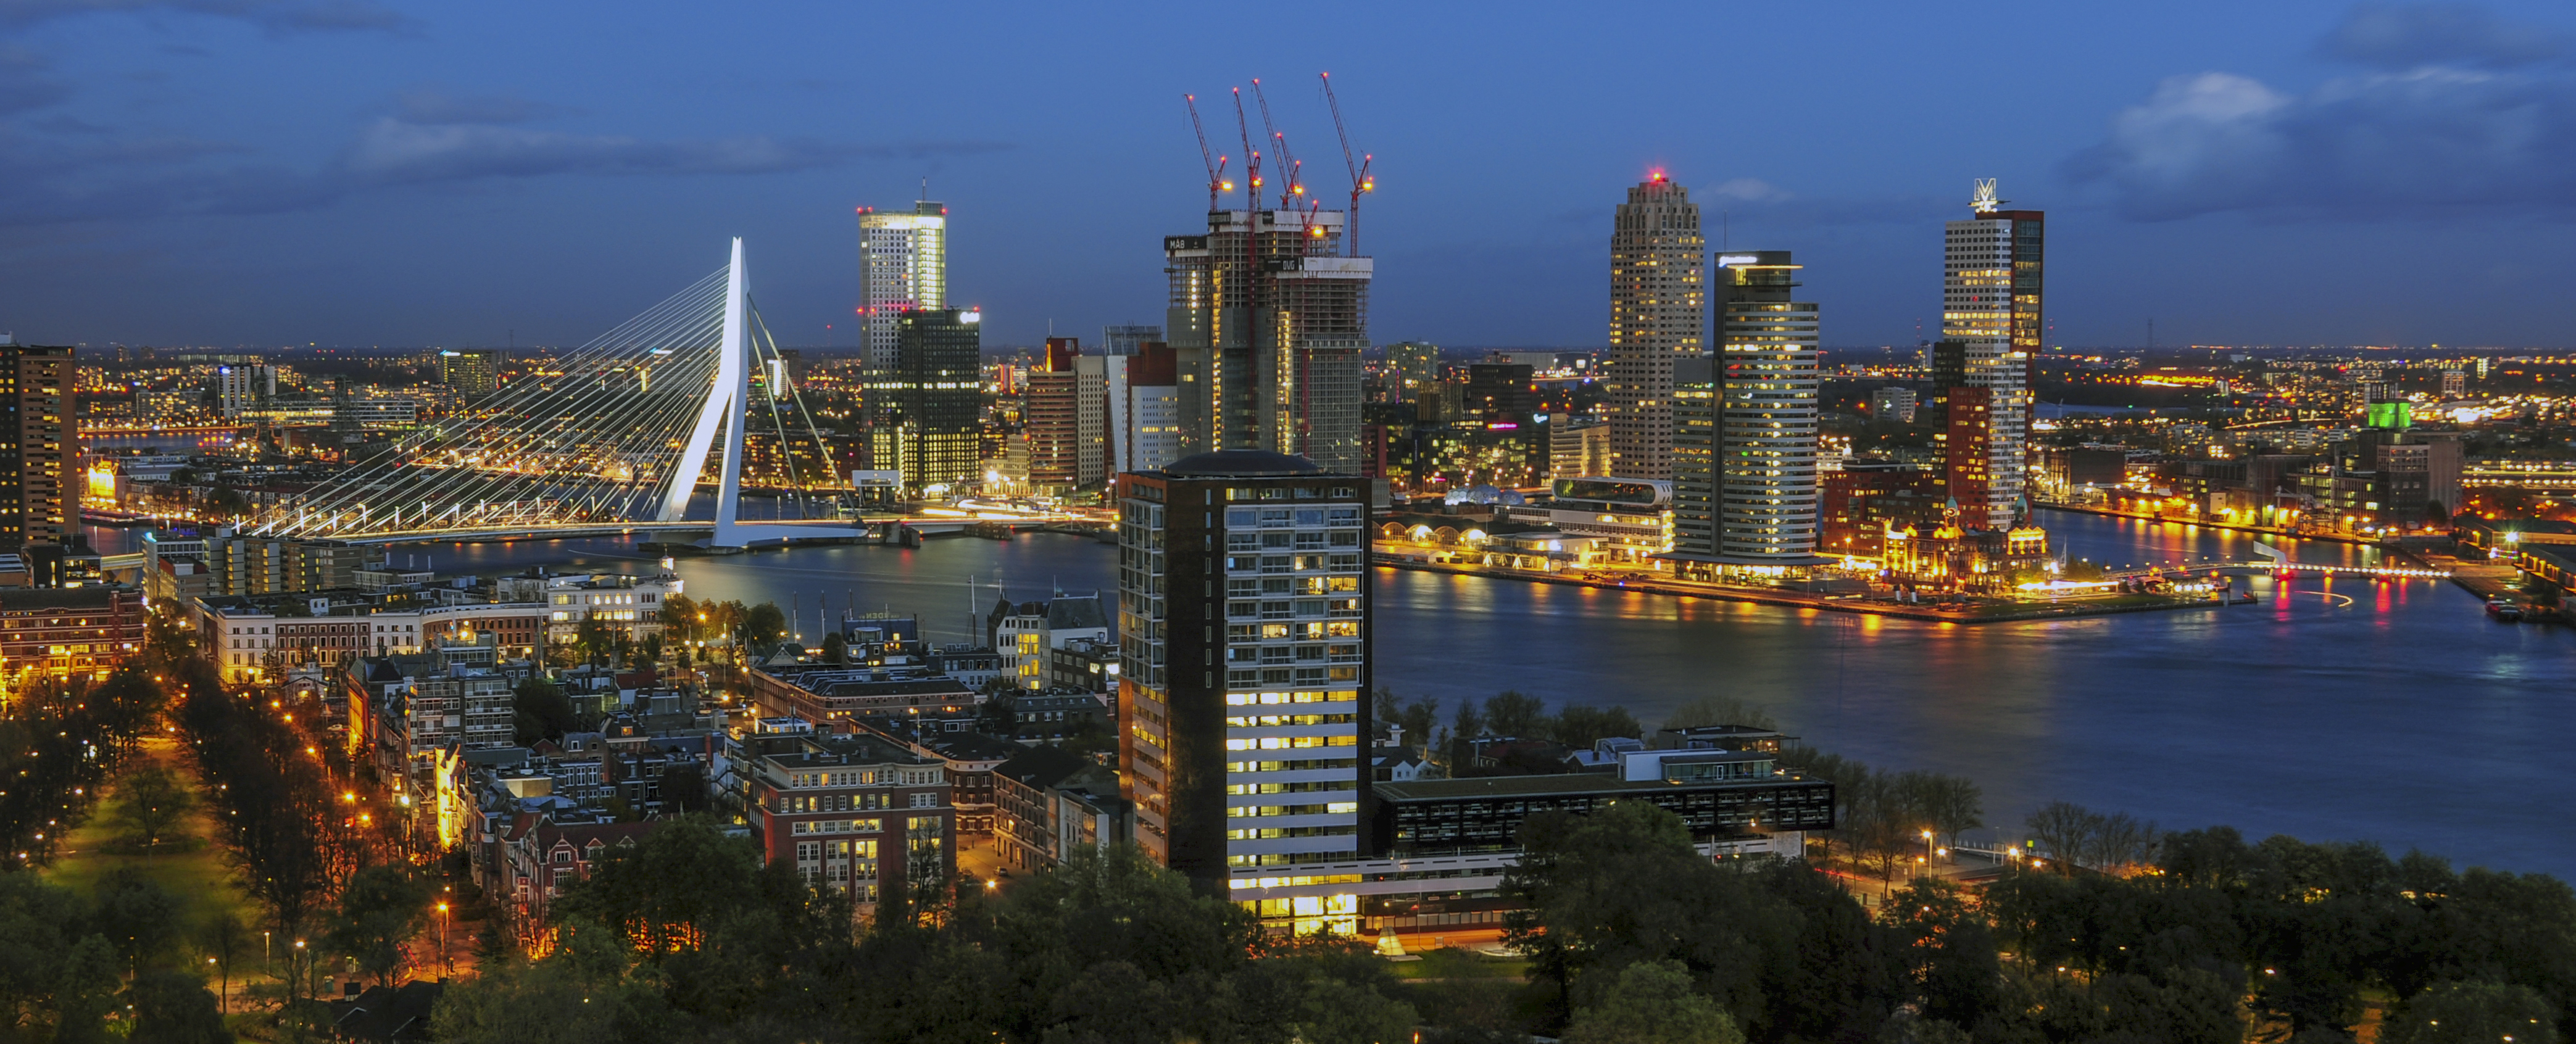
\includegraphics[width=\textwidth]{paper/imgs/Erasmusbrug_seen_from_Euromast.jpg}
% \end{figure}

\begin{abstract}
    In this paper, we present Route2Dam, a group travel recommender system for Utrecht University students that want to visit the city of Rotterdam. The system uses Gaussian processes and pairwise comparisons as a model-based approach to elicit preferences. 
    The preferences are used to construct individual and aggregated group recommendations. Furthermore, the system will adapt its recommendation on-site based on the current contextual aspects like time, location, and weather. The paper will provide insights into design decisions, the recommendation system, implementation details, and the intended user experience. 
\end{abstract}

\section{Introduction}
This paper will dive into one of the most popular leisure activities in the world -- travelling to new places.
Especially, over the past few decades the tourism sector saw substantial changes.\cite{smeral_StructuralViewTourism_2003}\cite{doi:10.18111/wtobarometereng.2020.18.1.1} Not only have the number of tourists constantly grown but the tourists themselves changed, too.\cite{OECD2020}
In particular, young travellers are increasingly diverse; They display varying preference traits, and tourism suppliers must adapt to the needs of digital natives to remain relevant.\cite{europeantravelcommission_StudyGenerationTravellers_2020}  To face these challenges, one must be aware of current developments in E-tourism, which currently focuses on mobile tourism as smartphones provide more flexible ways to experience the travel destination than simple websites.\cite{mobile_recommendation_systems} This paper will introduce Route2Dam, a mobile group tourist recommender system, providing sightseeing recommendations on day trips based on the young people's profiles, needs, and goals. 

\section{Design}
\label{sec:design}
Route2Dam is an application which recommends various activities to groups on a single day trip in Rotterdam. This general goal helps to place the application in the broader taxonomy of tourism. Not only will the application deal with the type of tourism \citeauthor{dunnross_SightseeingTouristsMotivation_1991} call 'sightseeing' but we can even place the application in a subcategory called 'city-tours'. This categorisation helps us to make assumptions about the users and the context in which they operate. The next sections will explain how the users of the system are characterized and the important contextual aspects that influences their experience. 
\subsection{User Modeling}
\label{sec:UM}
Knowing that the application not only operates in the domain of city tours, but that the main users are students from the Utrecht University, helps formulating a representative user model for the application. In the following, we will explain who the user is, how the application models the users' preference and how the application adapts to the users' characteristics. 

\subsubsection{Characterizing the individual and the group}
As mentioned earlier, the goal of our application is to provide optimal guidance to groups of students visiting Rotterdam for a day trip. However, we have to rely on information about individual users to come up with a recommendation that fits the group. Hence, it is necessary to characterize the expected users of the system. In our case, the targeted user is a student at Utrecht University. According to a study by \citeauthor{AgeAverage_students}, we can expect young students between 20-29 years old.\cite{AgeAverage_students} Most of them are digital natives and therefore, adept at using mobile applications.\cite{prensky_DigitalNativesDigital_2001a} Furthermore, we can assume the main goal for conducting a city-trip, includes the desire to experience a different lifestyle, the need to relax, or escaping the ordinary. Others are also interested in sightseeing and attending local events.\cite{rita2019millennials} For those who are primarily interested in the city, seeing most of Rotterdam's sites during the limited time is particularly important. Although most students of Utrecht University are Dutch, we can still assume that their different backgrounds and cultures vary significantly. This is supported by the \emph{Annual Report of Utrecht University 2019}, which states that 10\% of all students are international.\cite{utrecht_UniversiteitUtrecht_2019} Furthermore, even among Dutch students, we can expect an increasingly diverse population of students, as early trends of the dutch \emph{Centraal Bureau voor de Statistiek} suggest.\cite{theovanmiltenburg_AllochtonenHogerOnderwijs_2007} Hence, the application faces a multitude of preference profiles. Students are also expected to have a relatively low budget. Although, the average income varies strongly over household types (living with parents, a student house, own house/apartment), the average of €587 remains low.\cite{kobus_OwnershipOncampusUse_2013} Hence, we can assume a high sensitivity for extracurricular expenditures. Lastly, we can expect each user to lean towards certain activity types. These are categories of activities that share core characteristics, such as \emph{Museums}, \emph{Bars}, etc.. 

All these characteristics need to be considered if we want to understand a user's preference profile. However, some dynamics only occur within groups, which is why we also have to characterize how we define the notion of a group. We consider every set of users with a cardinality higher than one group. Additionally, we assume that the users of the application are acquainted with each other. This assumption simplifies the scope of the application in two ways. First, we do not have to introduce a person to person recommendation module. Second, we can expect communication outside of the application. However, this also introduces problems in group decision making like direct confrontations and peer pressure.\cite{asch_OpinionsSocialPressure_1955}\cite{gitelson_InfluenceFriendsRelatives_1995} This solidifies the need to find a consensus first or if that is not possible for anonymous voting mechanisms within the application.
For practical reasons, the application will also distinguish between the group's administrator and a regular user. The group administrator initiates the trip within the system by setting up the trip and inviting other group members. However, this distinction only stems from technical and procedural considerations, described later in the paper. Apart from these practical considerations, the group administrator is a regular user as established above. 
The application will retrieve basic personal information about each user of the group via the registration process. User accounts will be used to keep track of the individual user model, which contains a user's preferences and personal settings. The initial information is used to create a personal set of recommendations, which can be used for individual city-trips or as part of the group's trip recommendation.
  	
\subsubsection{User adaption and Preference Modeling}
As mentioned earlier, the application retrieves information about the user in order to suggest relevant guidance through Rotterdam. Two major components act as sources for this adaption process -- user characteristics and pairwise comparisons. 

The characteristics will act as input for the second component and are configurable by the user. We will use them to compose the user representation and compute user similarities. As a result, they will not influence the recommendations directly (with an exception for budget and history). The user characteristics consist of: 
\begin{itemize}
\item \textbf{Budget:} The student's income highly influences the set of activities the user can partake in. Therefore, the user will be asked to specify his travel budget which will subsequently filter the available recommendations. Budget is an exception among all other characteristics, as it will also act as a preliminary filter. As a result, it will influence the recommendation directly. More on that in \autoref{sec:rs}.

\item \textbf{Rotterdam first-timer:} The user can specify whether he has visited Rotterdam before or not. This will influence the recommendations the system provides. Users that have never visited Rotterdam will likely have different recommendation needs compared to users that are already acquainted with the city.

\item \textbf{Cultural background:} The application will query whether the user is Dutch or an international. The reason is internationals tend to visit places that are more suitable for expats, while Dutch user's are not constraint by language barriers.

\item \textbf{Associated faculty:} A student's study program acts as an indicator for preferring certain activity types over others. However, this is impractical to include in our model, as Utrecht University has too many study programs to encode within the system. It uses the associated faculty of the student as proxy.

\item \textbf{Activity type preference:} We can also gain knowledge about the user's activity type preference by tracing which types of activities the user prefers over others. This will be further detailed in \autoref{sec:impl}.

\item \textbf{History of visited activities:} As soon as users used the application once, we can store the places that they have visited. We can use this information as preliminary filter to avoid recommending the same activities multiple times.  
\end{itemize}


At this point, it is important to explain how the application collects information about the user's preference relations. In preference theory, an individual's preferences rely on a latent utility function.\cite{chen_SurveyPreferenceElicitation_2004} If one can uncover the utility function, one can also make statements about an individual's preference ranking over a set of alternatives. A naive approach would be to ask the user to score each possible alternative, but this would be too expensive for our application, given the number of activities and users.\cite{chajewska_MakingRationalDecisions_2000} Instead, we can rely on so called preference elicitation techniques to approximate the latent preference function of a user under the constraint of having minimal user signals. Pairwise comparisons are very suitable for this task for two reasons. Not only do they impose a very low cognitive burden on users, but it is also possible to retrieve a ranking of alternatives if enough comparisons are available.\cite{conitzer_ElicitingSinglePeakedPreferences_2009} We use these user signals to model the preferences of each user. After the preliminary filters are configured for the user, the system will start the process of users' preferences retrieving. The application starts by presenting two alternative activities to the user. The user will be asked to choose between them. The comparison result will be stored and used to infer a model about the user's preference function.\footnote{In order to avoid confusion, the comparison result mentioned here is different from the activity type preference that we will also retrieve from this process. It is important to understand, that pairwise comparisons not only provide information about preferred items over other items, but indirectly which activity types the user seems to prefer. The former will inform the model while the latter is used for the user representation.} \autoref{sec:adaptive_hm} will explain the process in detail while \autoref{sec:rs} explains the recommender system. 


\subsection{Context Model}
\label{sec:context}
Now that the previous section explained briefly how the model adapts to the user, it will be necessary to explain the context adaptation. Most of the adaptions described in this section will influence recommendations on-site, which contrasts user adaptions, which affect recommendations beforehand and remain static throughout the trip.

Being a recommender system for city-tour activities, the application has to place a particular importance to contextual aspects of the trip. Namely, the location, the time and the weather in which the application is used. In the next paragraphs, we are going to describe how the application manages to adapt to the context. \autoref{fig:adaptions} show cases the adaptions that take place.

\subsubsection{Weather}
The weather situation has always been an important tourism factor that requires special attention due to its unpredictable behaviour. Several studies show a specific need for adaptation, as it is a key driver for user satisfaction or dissatisfaction.\cite{becken_ImportanceClimateWeather_2010} Among others, \citeauthor{defreitas_TourismClimatologyEvaluating_2003} identifies two on-site behaviours that the application needs to take into account. Not only do tourists want to avoid unfavorable weather conditions (eg. move from sun to shade), but they change their activity accordingly to suit them (eg. swim more/less). 

Due to that, our application will retrieve weather-related information about the current location from online application interfaces such as \emph{openweathermap.com}. The location will be based on the longitude and latitude of the group's location. The administrator's GPS location, given by a mobile device, will be used as a proxy to represent the entire groups' location. We favor the geographic coordinates latitude and longitude, as they provide a more accurate retrieval of the current weather situation than the city or regional information about the weather. In fact, a big city like Rotterdam can experience various weather conditions in different parts of the city. 

As a result, the application will be able to filter options that are deemed unsuitable for the current weather condition. The system can, for instance, switch from outdoor activities to indoor activities and vice versa.\cite{creemers2015meteorological} This means that a park visit will not appear as an alternative during heavy rain, but indoor activities like museums or bar visits instead.

\subsubsection{Location}
The adaptation to location spans two dimensions: On the one hand, we identify a static dimension as the application is adapting to the city of Rotterdam. This will be covered in depth in \autoref{sec:UX}. On the other hand, there is a dynamic dimension as the location of the group within the city changes constantly from activity to activity. Here, the application requires special attention to spatial adaptation. The application can use GPS to locate the group's current location within the city. With this information, it is possible to adapt its recommendation in two ways. 

First, the application can provide ad-hoc recommendations for popular points of interest that are situated within a walking range of roughly 0.7km. We chose this heuristic based on the maximum distance that students in the Netherlands still consider a walkable distance.\cite{ton_CyclingWalkingDeterminants_2019} This is equivalent to a 10min. walk, given the average walking speed of healthy individuals (4.5km/h).\cite{schimpl_AssociationWalkingSpeed_2011} As an alternative, the application could also compute the average group walking speed, but this measure might be confounded by the nature of the current visited activity or the mode of transportation. Consequently, it was deemed unreliable. The "must-see"-locations will come in form of notifications which the group can choose to visit or ignore. 

The second application of location information relates to the group ranking, which will adapt based on the current location of the group. Here, the location will act as a weight for every item utility in the group recommendation list. The weighting follows the following formula.

\begin{equation}
    Utility_{i}^* = \frac{Utility_i}{\lvert Location_i - Location_G \rvert}
\end{equation}

Here, $Utility_i$ refers to the group's utility and $Location_i$ to the location of a particular item $i$, while $Location_G$ refers to the current location of the group. This re-weighting will start after the group's completion of the first activity on the recommended list. The reason for this decision is that earlier use of the location factor most likely leads to confusion because it causes unexplained changes in the ranking prior to the visit. 


\subsubsection{Time \& Date}
While weather and location can be considered \emph{soft filters} due to the group's ability to ignore these factors, the temporal context plays a crucial role in the accessibility of events, points of interest (POI) or activities. As an illustration, a group cannot choose to visit a location outside of its opening hours, and recommending such an item will most likely lead to strong dissatisfied responses. Hence, the application's recommendations must take temporal considerations into account. We can group these adaptation considerations based on the types of information that will be used. Namely, time, date, and the combination of both. 

As the date is specified by the group's administrator upon tour creation, we do not have to resort to specific methods to retrieve the information. Similar to location, we can use the date as a notifier for upcoming events. Unlike location, the event notification will not be on-site but prior to the tour date.

The current time finds its use in discriminating between morning, daytime and nighttime activities. For that purpose we can leverage the system time of the group administrator's smartphone. This will allow the application to favor activities suitable for the current time of the day.

The conjunction of date and time will mainly be used to filter out activities that are not accessible. Although simple in theory, there are more additional practical considerations to take into account. First, the group must be able to reach the activity on time. Second, the group should not arrive shortly before the activity closes. The former is simple to compute, using the average walking speed of healthy individuals of 4.5km/h and the distance between the location and group. Walking is the slowest mode of transportation and thus guarantees that the group will reach the activity and have enough time. 

The latter, however, highly depends on the nature of the activity. For instance, a study by \citeauthor{serrell_PayingAttentionDuration_1997} found that most people spend approximately less than 20 minutes in a museum regardless of exhibitions size, while staying in bars differs significantly by type according to \citeauthor{harford_DrinkingBarsObservational_1983}.\cite{serrell_PayingAttentionDuration_1997}\cite{harford_DrinkingBarsObservational_1983} We chose to use the simple heuristic of the average time spent in a location. We can use the \emph{Google Maps API} to retrieve the information, resulting in the utility assignments. 
\begin{equation}
    \forall i \in A: T_i - (T_{now} + \frac{\lvert Location_i - Location_G \rvert}{4.5}) < \overline{T_i} \Rightarrow Utility_{i}^* = 0
\end{equation}
$T_i$ refers to the closing time of activity $i$ in the set of all activities $O$. $T_{now}$ refers to the current time. Like with location, this update only occurs after visiting the first activity. 

% TODO: Fix this
\begin{figure}[H]
    \centering
    \subfloat[\centering]{{\includegraphics[width=0.20\textwidth]{paper/imgs/hifi_prototypes/beach.png} }}%
    \subfloat[\centering]{{\includegraphics[width=0.20\textwidth]{paper/imgs/hifi_prototypes/cinema.png} }}%
    \qquad
    \subfloat[\centering]{{\includegraphics[width=0.20\textwidth]{paper/imgs/hifi_prototypes/brunch.png} }}%
    \subfloat[\centering]{{\includegraphics[width=0.20\textwidth]{paper/imgs/hifi_prototypes/bars.png} }}%
    \qquad
    \subfloat[\centering]{{\includegraphics[width=0.55\textwidth]{paper/imgs/hifi_prototypes/location_adaptation_combined.png} }}%
    \caption{Show case of different context adaptations: First, outdoor and indoor adaptations because of weather changes (a \& b). Second, day-time and night-time activities based on the current time (c \& d). Third, closely located activities are higher ranked (e). 
    }%
    \label{fig:adaptions}%
\end{figure}

\subsubsection{Rotterdam}
The last context, which is often overlooked, is the adaptation to Rotterdam, the former European cultural capital.\cite{hitters_SocialPoliticalConstruction_2000} After its destruction in WW2, Rotterdam's tourism primarily focused on modern culture.\cite{rotterdam} The result of that was a modernistic architecture, which shifts away from the traditional Dutch model. The application's adaption to Rotterdam is an inherent part of design goals with regard to visuals and content. For instance, the application's name \emph{Route2Dam} is a wordplay, as it bears acoustic resemblance to \emph{Rotterdam}. In terms of content, the application assumes that the students will not change the location during the day trip which is why the application only shows locations and events confined to Rotterdam. Other locations are excluded. The user interface (UI) of the application was created with Rotterdam's modernistic architectural design in mind. An example of this can be seen in the splash screen, which shows the \emph{Erasmus Bridge's} silhouette. However, more details about visual design decisions are going to be elaborated in the UI section of this paper.

\section{Adaptive Hypermedia}
\label{sec:adaptive_hm}
The adaptive hypermedia part of the system revolves around the pairwise comparison. Our system will show each user a different pair of items to compare depending on his selection. This procedure resembles the way other adaptive hypermedia systems show different content, depending on the order of the links that have been clicked. Thus, this section will explain how items are presented towards the user and how they are initially chosen. 

\subsection{Presentation of Pairwise Comparisons}
As mentioned in \autoref{sec:UM}, this system will use a series of pairwise comparisons to model the preferences of a user. These pairwise comparisons are presented in the form of two items being shown on the screen. It has long been known that users find choosing between two items easier than choosing among a set of options. The user will then be able to click on either of the items. Clicking an item is equivalent to stating that the clicked item is preferred over the alternative. Subsequently, the user will have to answer the next pairwise comparison query. This querying process repeats at least three times. Afterwards the user is free to either compare more items or to end the process. With more comparison, the resulting ordering of the activities will be closer and closer to the optimal one, assuming at least one optimal ordering exists for a specific user.

There are two alternatives to the approach of showing the next queries: either replacing the unpreferred activity with a new item or letting the user choose among two completely new items. 

The last option may provide the opportunity to explore the latent preference function more, as we can sample items from different parts of the items space. However, unlike with the former alternatives, we cannot leverage a crucial advantage of preference relations -- the transitivity of preference alternatives.

The rule states, that if the item a is preferred over item b and item b is preferred over item c, then under the assumption of preference consistency the user also prefers item a over c. Meaning, we attain three pairwise comparison results from asking two comparison queries. However, this approach also comes with problems, due to its consistency assumption. We cannot always assume that the user will answer consistently.

The application will employ the latter option, as it allows to exploit transitivity to gain more knowledge about the user. Although consistency being a strong and unlikely assumption, the probablistic nature of the pairwise-comparison model mitigates the uncertainty arising from inconsistent query responses.
In \autoref{fig:pairing_process}, we show the full process.
\begin{figure}[H]
    \centering
    \includegraphics[width=\textwidth]{paper/imgs/pairwise_comparisons.png}
    \caption{Simplified illustration of the pairwise comparison process in and how it results in an individual ranking for the user.}
    \label{fig:pairing_process}
\end{figure}

\subsection{Query Pair Selection}
\label{sec:pair}
Now that we have explained how the queries are presented two questions remain: How do we select the individual pairs and how can we use the query results to recommend an ordered list of activities? In this section, we will answer the former question, while the latter will be answered in \autoref{sec:rs}. 

As mentioned prior, the application needs to select different pairs of items based on former query responses. Given that we do not know anything about the user's preferences at the beginning, we first have to explore the space of possible preferences as much as possible. The application achieves this by querying pairs that are diametrically opposed. Starting with a randomly selected activity, the application chooses another activity that maximizes the dissimilarity between both activities. As every activity is represented as vector, we are free to use any vector similarity metric such as the cosine similarity or any Minkovski distance (e.g.: Euclidian distance). However, after the first query result, we cannot rely on this method anymore, as the next maximally dissimilar item would be very similar to the item that vanished after the first decision. In other words, we need to query for an item that is maximally dissimilar to the first pair. For that purpose, we can find the activity that is the most similar to the cross product of both activity vectors. Mathematically, the cross-product of two vectors yields a vector that is linearly independent from both initial vectors. To be more specific, the cross-product has a 90° degree angle to the plane that both vectors form and is maximally dissimilar to both if we consider the angle as measure for similarity. As a result, we will apply cosine similarity consistently as similarity measure for all activities as it relates to the angle between vectors. \autoref{fig:item_vectors} illustrates the above reasoning. After explaining the decision for the first two query pairings, we can now repeat the established process. 

\begin{figure}[H]
    \centering
    \includegraphics[width=0.75\textwidth]{paper/imgs/geogebra-export.png}
    \caption{Image shows three activities (red, blue, green) represented as vectors. The red activity and the blue are dissimilar as their angle is large. Both vectors span a plane, whose normal vector we can compute with the cross product. We can find the next activity by finding the activity whose angle is closest to the cross product. In this example, that would apply to the third activity (green)}
    \label{fig:item_vectors}
\end{figure}

This approach is viable for exploring multiple opposing angles of preferences. However, as mentioned above, we also have to elicit the intricacies between activities that are roughly similar but differ in detail. A user might like going to museums, but may prefer a contemporary arts museum over a natural history museum. The simplest solution is alternating the aforementioned procedure with one that picks a similar activity as next query partner. As stated before, we start with the alternation after the third query response. 



\section{Recommender System}
\label{sec:rs}
The recommender system will provide the users with a way to settle on a common itinerary for a day trip to Rotterdam. The system will achieve its goal by taking into account concepts like privacy, social pressure, and cognitive overload. The users interact with the system through an application installed on their personal mobile phones. By having the application, the users can decide independently about their preferences and expectations regarding the trip. In this manner, we guaranty privacy and avoidance of social pressure. The group recommendation system uses an egalitarian approach to aggregate the preferences and generate the group recommendations. When aggregating, this approach is achieved by attributing the same weight to each individual ranking and not balancing by taking into account the number of queries to which each user responded.

The recommender system can be thought of as a pipeline of 3 independent components. The first component (\emph{Individual User Recommendations Component}) will take the preferences of a user and convert them into a personal ranking of possible activities. This is achieved by framing the problem as a preference elicitation problem with a focus on using pair wise comparisons. Having generated the individual rankings for all the members of a group, the second component (\emph{Ranking Aggregation Component}) will then aggregate the rankings into a group ranking of possible activities. At this point, the users will choose an item from the ranking and the third component (\emph{Routing Component}) will use route recommendation techniques to guide the group towards the location of the chosen activity. Outside of the 3 components, a set of \emph{preliminary filters} will be applied to the activities before entering the pipeline. Each component will be discussed in detail in the following subsections.

\begin{figure}[H]
    \centering
    \includegraphics[width=0.8\textwidth]{paper/imgs/chart_ais.png}
    \caption{The simplified pipeline including the main components of the Recommender System described in this section}
    \label{fig:pipeline}
\end{figure}

\subsection{Preliminary Filters}
The system discards some activities from the list by applying preliminary filters. Those filters are the date of the trip, the maximum budget set by the user, the start hour of the trip, and previously visited activities. These preliminary filters are backed up by simple assumptions that might improve the overall experience. If all the group members have a maximum budget of \EUR{40}, it does not make sense for the system to include events that are more expensive than \EUR{40}. It is also beneficial to exclude activities in a location that are closed before the start time of the trip. Similar reasoning can be applied to previously visited locations, as we can expect, that most individuals do not want to see the same location recommended a multitude of times. Applying these filters will remove inconsistent activities and redundancies leading to a simplified recommendation process.

\subsection{Individual User Recommendations}
The system has access to a vast list of activities that can be attended in Rotterdam. The goal of the \emph{Individual User Recommendation} component is to sort this list according to the user's preferences, thus creating a desirable ranking of activities. The ranking will be generated using pairwise comparisons, or \emph{queries}. In the case of our system, a query is represented by presenting two specific activities to the users from which they will choose the one that suits them the most. From this choice, order can be inferred for the two alternatives; activity $i$ is preferred over activity $j$: $q_{i,j} = a_i < a_j$.  We would have to query $O(n\cdot log(n))$, assuming consistent answers from the user; $n$ is the number of activities in the list. However, as we do not want to demand too many queries responses from the user and considering the fact that any preference ranking can be equated by a utility function defined on the domain of preferences, we will make use of introduced uncertainty and treat the problem as a \emph{preference elicitation problem}. We will use the Gaussian Process Preference Elicitation approach described by \citeauthor{guo_GaussianProcessPreference_2010} \cite{guo_GaussianProcessPreference_2010} to derive the result of new queries without the user's input. Our choice is supported by the non-parametric Bayesian nature of Gaussian Processes which translates in having a flexible model of user's utility. The model works under uncertainty and can easily integrate new information. The model also proves to be more efficient than a classical content/user filtering recommender system which assumes a large user-base. This is supported by the inner workings of the system that can automatically handle the cold-start problem present in other recommender systems.

As mentioned above, we will model the utility function using a Gaussian Process having the following form:
\begin{equation}
    \label{gp}
    f(u, a) \sim GP(0, k^u(u,u')k^a(a, a'))
\end{equation}
$a$ and $a'$ are two different activities. Same holds for $u$ and $u'$ as two distinct users. $k^u$ and $k^a$ are the covariance functions on the user feature vectors and, respectively, the activity feature vectors. Each covariance function, or \textbf{kernel}, comes with its own hyperparameters ($\theta$) used in regression settings.

We assume the users' preferences to be conditionally independent as we consider the theoretical best-case scenario in which the users will not be influenced by external parties in stating their personal preferences and self-applied restrictions, thus excluding social pressure and group bias. Under this assumption we model the probability of a user $u$ to prefer an activity $a$ over $a'$ as shown in equation \ref{eqm}, where $f$ is the previously mentioned utility function.
\begin{equation}
    \label{eqm}
    p(a^u > a'^u | f(u,a) - f(u,a'), \xi) = I[\xi \leq f(u,a) - f(u,a')]
\end{equation}
Here, $\xi$ is a normally distributed variable which guides the value of $f$ such that the stated relation holds. $\xi$ simply captures the introduced noise variation. $I$ has value $1$ if $\xi \leq f(u,a) - f(u,a')$ is true and $0$ otherwise. Following the paper, from \ref{eqm}, we can deduce the respective normal cumulative distribution function and the probability of having some observations given the utility function $f$:
\begin{equation}
    \label{eqm}
    p(O|f) = \prod_i^U \prod_{j, j'}^A \frac{1}{\sigma} (f(u^i, a^i_j) - f(u^i, a^i_{j'})) 
\end{equation}
where $U$ is the set of users, $O$ are the observed query results, $A$ is the set of activities and $\sigma$ is the standard deviation of $\xi$. 

Now we can model the posterior and predictive distributions using the Bayesian Inference formula in equation \ref{bayes}, where $f$ is again the utility function, and $\theta$ stands for the kernel hyperparameters.
\begin{equation}
    \label{bayes}
    p(f|O, \theta) = \frac{p(O|f,\theta) \cdot p(f|\theta)}{p(O|\theta)} 
\end{equation}
Equations \ref{posterior} and \ref{predictive} show the resulted posterior and predictive distributions. The posterior distribution was calculated by a Laplace approximation followed by an iterative application of the Newton's method to derive the maximum posterior $f_{max}$.
\begin{equation}
    \label{posterior}
    p(f|O) = N(f|f_{max}, (W + \Sigma^{-1})^{-1})
\end{equation}
\begin{equation}
     \Sigma = K^u \otimes K^a
\end{equation}
where $\otimes$ is the Kronecker product between the covariance between all the user vectors $K^u$ and the covariance between all the activities vectors $K^a$; $W$ is the ratio between the function and the first derivative of the function present in Newton's method iterative approach. The predictive distribution from \ref{predictive} will be use to elicit the preferences of an user $u^*$ over two unseen activities $a^*_1$ and $a^*_2$. 
\begin{subequations}
\label{eqn:preddist}
\begin{equation}
    \label{predictive}
    p(f^*|O) = N(f^*|\mu^*, C^*)
\end{equation}
\begin{equation}
    \mu^* = (K^*)^T\Sigma^{-1}f_{max}
\end{equation}
\begin{equation}
    C^* = \Sigma^* - (K^*)^T(\Sigma - W^{-1})^{-1}K^*    
\end{equation}
\end{subequations}

\autoref{eqn:preddist} shows that we only have to compute $\mu^*$ to get an estimate for the unknown values in $f^*$. The computed covariance $C^*$ is not necessarily required for the application but it provides us with the level of uncertainty for the estimation.
 
\begin{subequations}
    \label{eqn:computation}
    \begin{equation}
         K^* = (K^*)^u \otimes (K^*)^a
    \end{equation}
    \begin{equation}
         (K^*)^u = [k^u(u^*, u_1),\hspace{5} ...\hspace{5} k^u(u^*, u_{|U|})]
    \end{equation}
    \begin{equation}
         (K^*)^a = \begin{bmatrix}
       k^a(a^*_1, a_1),  \hspace{5}...\hspace{5}  k^a(a^*_1, a_{|A|}) \\
       k^a(a^*_2, a_1),  \hspace{5}...\hspace{5}  k^a(a^*_2, a_{|A|})
       \end{bmatrix}
    \end{equation}
    \begin{equation}
         \Sigma^* = \begin{bmatrix}
       k^u(u^*,u^*)k^x(a^*_1, a^*_1) &
       k^u(u^*,u^*)k^x(a^*_1, a^*_2) \\
       k^u(u^*,u^*)k^x(a^*_2, a^*_1) &
       k^u(u^*,u^*)k^x(a^*_2, a^*_2) 
       \end{bmatrix}
    \end{equation}
\end{subequations}
We can use the described process to find the most k preferred activities for every user. Hence, we also provide individual recommendations, even if the macro system is defined for group recommendations. 


\subsection{Ranking Aggregation}
Having obtained the rankings for all the users, we will need a method to easily aggregate them into a group ranking. Here we will make use of the game theoretic notion of social choice. More specifically, we will use Borda voting.\cite[p. 257]{shohamMultiagentSystemsAlgorithmic} Borda voting functions by taking the fully ordered list of preferences of each user and assigning points in descending order from the top preference to the lowest-ranked preference. This can be further illustrated by a simplified example. 
Assume we have a group of 3 users \{$u_1$, $u_2$, $u_3$\} and 4 possible activities (after filtering) \{$a_1$, $a_2$, $a_3$, $a_4$\}. Consider the following resulted individual rankings: $u_1$ : $a_1 > a_2 > a_3 > a_4$, $u_2$ : $a_3 > a_2 > a_1 > a_4$, and $u_3$ : $a_2 > a_3 > a_4 > a_1$. This will translate to the following Borda voting vectors: \\
\begin{center}
    \begin{matrix}
    A \\
    a_1: \\
    a_2: \\
    a_3: \\
    a_4: \\
    \end{matrix}
    \begin{matrix}
    u_1 \\
    3 \\
    2 \\
    1 \\
    0 \\
    \end{matrix}
    \begin{matrix}
    u_2 \\
    1 \\
    2 \\
    3 \\
    0 \\
    \end{matrix}
    \begin{matrix}
    u_3 \\
    0 \\
    3 \\
    2 \\
    1 \\
    \end{matrix}  
\end{center}

From here, we can obtain the group ranking by adding the vectors together:

\begin{equation}
    \begin{bmatrix}
    3 \\
    2 \\
    1 \\
    0 \\
    \end{bmatrix} + 
    \begin{bmatrix}
    1 \\
    2 \\
    3 \\
    0 \\
    \end{bmatrix} + 
    \begin{bmatrix}
    0 \\
    3 \\
    2 \\
    1 \\
    \end{bmatrix} = 
    \begin{bmatrix}
    4 \\
    7 \\
    6 \\
    1 \\
    \end{bmatrix}
\end{equation}
This vector now translates back to the group ranking of activities $a_2 > a_3 > a_1 > a_4$.

Borda voting, like any other voting schemes, cannot satisfy all notions of fairness (Arrow's Theorem).\cite[pp. 260]{shohamMultiagentSystemsAlgorithmic} This comes as a general theoretical disadvantage, but one that can be balanced by computational advantages. We use Borda voting as we have direct access to the sorted list of each group member as soon as the execution of the first pipeline component is ready. Another reason that supports using Borda voting lays in the fact that it provides a very fast preference aggregation in the form of adding $|U|$ ($U$ is the set of users) vectors which can be done in $O(1)$ time. Because all the necessary operations are vector additions, the input of the aggregation component does not introduce a computational bottleneck. The vectors can be added in any order and there is no need to pausing the execution in order to collect the resulted data from all the users.

\subsection{Routing}
\label{sec:routing}
Two scenarios are possible after the computation of the group aggregate ranking of activities: creating a \textbf{visiting plan} including all the recommendations in the top-k ranking or choosing a \textbf{first destination} on which the group agrees. Both scenarios will be further described next, in reverse order. 
Subsection \ref{sec:context} already described an online adaptation based on location, distance, and budget. However, this adaptation begins after the first activity was finished. Being presented with the top-k ranking, the group must decide on the starting activity. Under the assumption that the system will be used by a group of friends, this could be done by an in person negotiation and argumentation. Even so, it can happen that the group is unable to reach a unanimous decision or several people refuse to take part in the negotiation. For these reasons, we propose a simple solution. The group will be presented with a new voting round. As we are now in a ranking system setting, approval voting is a good candidate for this scenario as \emph{Arrow's impossibility theorem} does not hold in this case.\cite[p. 257,267]{shohamMultiagentSystemsAlgorithmic} After computing the winner of the vote, each member of the group will be redirected to their default navigation application in which a route to the location of the desired activity will be presented. After having finished the first activity, the ranked list of activities will be updated. As the adaptation techniques described in \autoref{sec:context} work with real values, rather than ordered lists, the list will be min-max normalized such that any position in the list will have an utility between $0$ and $1$.

The second scenario translates in a visiting plan tailored for the day trip. If the members of the group are happy with all the top-k recommendations, the system can create a route that includes all of them. Each activity will be treated as a node in a complete weighted directed graph. A dummy start node that has only out edges will also be added. The weight of each incoming edge to a node will be a combination between the geographical distance of the source node and the destination node, the average time spent in the destination node, and the expenses attributed to the activity represented by that node. To arrive at a formula for computing the weights based on previously mentioned 3 arguments, a couple of assumptions will be made. A minimum geographical distance to the activity is desirable. Lower expenses are preferable over higher expenses. Even more precisely, lower expenses for an activity which can be enjoyed longer are preferred over higher expenses for an activity that has a shorter time frame. This assumptions have been summarized in \autoref{eqn:weights}.
\begin{equation}
    \label{eqn:weights}
    w = d + m \cdot (1 - t)
\end{equation}
Several things must be mentioned here. Firstly, $w$ stands for the weight, $d$ is the geographical distance, $t$ is the time frame, whilst $m$ represents the amount of money. Secondly, all the values that enter the formula have been min-max normalized in advanced, thus we deal only with values in the $[0, 1]$ interval. Lastly, as we model this as a shortest path problem, the lower the weight, the better. At this point we have constructed the graph. Evidently, calculating a path through all the activity nodes, without visiting two nodes twice happens to be the well-studied \textbf{Travelling Salesman Problem}(TSP). We deal with an NP-hard problem, in which a solution can be achieved, without using stochastic methods. The worst-case time complexity of $O(2^nn^2)$ and space complexity of $O(2^nn)$. However, we must remember that we are dealing with a graph with $k+1$ nodes, where k is a very small number (a one digit number). This implies that we can solve the problem using the Held-Karp algorithm, thus providing a well-adjusted visiting plan for the group.\cite{held_DynamicProgrammingApproach_1962}

\subsection{The Cold-Start Problem and Serendipity}
The cold-start problem and serendipity are among the most important aspects of recommender systems to address. 

The cold-start problem refers to the issue of adding a new user or item to the recommendation engine and incorporating it in the recommending process. In the case of users, the issue arises because of the lack of an initial understanding of the user's preference and subsequently the issue of recommending items without having that very knowledge. Similarly, in the case of newly added items, we have to question whether the item will be recommended. In typical recommender systems, we require interactions with the form of ratings, usage, etc. to characterize the item. If they are not available because the item is novel, we cannot recommend it. However, both cases are covered by the model based approach chosen in this paper. Because the model intrinsically compares the users' and items' similarity, it automatically generalizes them. Therefore, the recommendations will be similar for users and items that are alike, even if there has not been any user or item interaction, so far. 

Serendipity is another issue, that needs to be dealt by every recommender system, as they should display relevant novelty in its recommendations. This is particularly important for travel recommender systems since exploration is one of the main goals for using such systems. Two factors help Route2Dam to provide novel recommendations. The first factor stems from the probabilistic nature of the model. As shown in \autoref{eqm}, we include a configurable noise parameter in the model, ensuring that recommendations are never the same. Second, the history of the users former visits to Rotterdam. The application excludes formerly visited activities from being included in the individual recommendations.  


\section{Implementation}
\label{sec:impl}
Most of the descriptions so far have been mostly conceptually or visually informed. However, in order to get a holistic understanding of our application, we need to provide more information behind certain processes and formulas.

\subsection{Content and User representation}
A very important part of every model-based system is the representation of real-world objects within the system. For our purpose, we need to clarify the representation of users and activities in our system. As mentioned prior, both objects are represented as vectors. In the case of users $U = {u_1, u_2, \ldots, u_n} $ being vectors in $\mathbb{R}^d$. Dimensionality $d$ corresponds with the user's characteristics. Namely, cultural background, visiting history, budget, faculty and activity type preferences. Cultural background is a categorical and will be represented as dichotomous variable being either 0 for International or 1 for Dutch. Similar holds for visiting history as we only track whether the user has visited Rotterdam at least once (as 1) or never (as 0). Budget is a ratio variable starting from 0 to $+\infty$, but it will be normalized across all users of the system.\footnote{In practise, we have a maximum value for the budget as $\infty$ would introduce implementation errors.} Next, we include the faculty of the student as categorical variable. In the case of Utrecht University, this adds seven additional dummy-encoded variables plus one for non-students. Every user can only be part of one faculty. The activity type preference is a nominal variable ranging over the taxonomy of attraction groups and restaurant subcategories established by \emph{TripAdvisor}.\cite{tripadvisorllc_ContentAPIBusiness_2020} This results in 23 categories that can characterize the attraction preference of a user for a certain type of attraction. Each category leads to a corresponding dimension which can range over \mathbb{N}. Each dimension will track the count for which a user preferred a certain activity type by choosing an item in the pairwise-comparison process. 
To get a better understanding, it is important to note that we use the same 23 categories to represent an item for the recommender model. The only difference here is that each dimension is a dichotomous variable and every item can belong to $m$ categories. Furthermore, we include the average cost as a variable ranging from 0 to $+\infty$. In order to capture the context dimension we additionally include weather suitability, location, average activity duration and opening hours. Weather is a dummy encoded categorical variable whose dimensions indicate suitability for various weather characteristics. The weather dimensions are sun, clouded, rain, warm, mild and cold. Each item may be suitable for one or more weather characteristics. For location, the application stores the latitude and longitude of the activity, which range from -90 to 90 and -180 to 180 respectively. The average activity duration is a real valued variable. The opening hours consist of two variables -- start and end time. These values are stored in minute of the day. Meaning, both range from 0 to 1440. Activities that are accessible at all time will occupy the full range. Similar to the budget variable, all real-valued item variables will be normalized. To get a better understanding, here, a simplified and unnormalised example:
Let us consider an international user that has never been to Rotterdam before, and has a budget of \EUR{60}. Furthermore, the user has preferred museums three times over the alternative. A row vector covering these 4 dimensions will have the form $u = \left(\begin{smallmatrix} 1, & 0, & 60, & 3 \end{smallmatrix}\right)$. The item vector construction follows the same logic. 

\subsection{Pairwise-comparison model computation}
Given the set of users $U$, items $A$ and a dataset of pairwise comparisons $O$, we can now compute the preference models. For that purpose we have to specify a covariance function $k$, which captures the distance between items and users. Any Mercer-kernel function can be used, but as \citeauthor{guo_GaussianProcessPreference_2010} showed, the standard RBF-kernel suffices. The equation follows 

\begin{equation}
k(x, x') = \exp\left(-\frac{|| x - x' ||^2}{2\sigma^2}\right)
\end{equation}

where $\sigma$ is a hyperparameter that needs to be tuned with hyperparameter optimization techniques. $x$ and $x'$ are vectors which correspond to two user vectors $u$ or two activity vectors $a$. Knowing this, we can compute the quantities $K^*$ and $\Sigma^*$ of \autoref{eqn:computation} to find $\mu^*$ and $C^*$ with \autoref{eqn:preddist}. Having $\mu^*$ and $C^*$, constructing an approximate ranking is trivial. 

\subsection{Graph representation}
\begin{figure}[H]
    \centering
    \includegraphics[width=0.7\textwidth]{paper/imgs/graph.png}
    \caption{Visualization of a simplified visiting plan graph with 3 nodes + 1 dummy node}
    \label{fig:graph}
\end{figure}
This subsection will further detail the graph representation presented in \autoref{sec:routing}. We define the graph $G = (V, E)$. Every activity in the top-k group ranking is represented by a vertex (or node). To this we append a dummy node as the start node. In the case of \autoref{fig:graph}, $V = \{"Op Het Dak"$, $"Krunsthal Museum"$, $"Markthal"$, $"Train Station (Dummy)"\}$. We add the dummy node to compute a variation of the TSP problem where the start point does not need to also be the end point. In the implementation, we assume the arrows pointing at the dummy node to have $0$ weight. This is the reason why there are no arrows pointing at the dummy node in \autoref{fig:graph}. The graph is a complete graph. There are $|E| = n \cdot (n - 1)$ directed edges in the graph. From all edges, $n - 1$ edges which point to the dummy node have weight $0$. The reason why the graph is not an undirected graph is that each pointing edge depends on the information relevant to the activity it points to. Following \autoref{eqn:weights}, even if the geographical distance between \emph{Op Het Dak} and \emph{Markthal} is the same, the term dependent on time and money will have a different value for \emph{Op Het Dak} than for \emph{Markthal}. For the purpose of this problem, it is not important how the graph is stored into memory (either using an adjacency list or a matrix).

\subsection{Held-Karp Algorithm}
The Held-Karp Algorithm is a dynamic programming algorithm proposed in 1962 by \citeauthor{held_DynamicProgrammingApproach_1962} to solve the Travelling Salesman Problem and its variations. One of the variations is the Asymmetric Travelling Salesman Problem (aTSP) -- the one we model for the routing component of this project.\cite{held_DynamicProgrammingApproach_1962} This algorithm is an improvement on the brute force approach of computing the minimum tour by considering the cost for each path represented by a permutation of the nodes ($O(n!) \approx \sqrt{2 \pi n}(\frac{n}{e})^n$ time complexity using Stirling's approximation).

As every dynamic programming approach, the Held-Karp algorithm decomposes the problem into sub-problems which are correctly solved through exhaustive search. Be $C_\pi$ the cost (total weight) of the path $\pi$. It follows that the algorithm is trying to achieve the minimization of $\sum_{p \in P}C_p$. For simplicity, we assume the nodes in the graph to be numbered from $1$ to $j$. We note $C_{S, j}$ the minimum cost cycle-free path from the start node ($1$) to the end node ($j$) and visits all the nodes in the set $S$. Using this notation we can write the recursive formula at the base of the algorithm, in which $V$ is the set of all nodes:
\begin{equation}
C_{S, j} = min_{k \in V - \{1, j\}}(C_{V - \{j\}, k} + C_{kj})
\end{equation}
The same formula will be recursively applied for $C_{V - \{j\}, k}$, which is already the minimum cost path up to this point, while calculating the minimum is done by exhaustive search. The implementation will require all the solutions of the sub-problems to be stored ($O(n2^n)$ space complexity). The time complexity of Held-Karp is $O(n^22^n)$. Even if the time complexity was reduced from factorial to exponential, it still remained inside the class of exponential-time problems. However, in our case, $n < 10$, therefore the Held-Karp algorithm can still be applied successfully.

\subsection{Procedural flow of usage}
Now that this paper has explained all the components of Route2Dam in isolation,
\autoref{fig:flowchart1} shows the full interaction of these components in a holistic process chart. The process is composed of 4 stages: “Group Formation”, “Pairwise comparison”, “Admin proposal” and “Voting”. The system knows two user roles: The \emph{Group Administrator} is the user who has set up the city-trip, giving him additional privileges. \emph{All Group Members} are composed of the remaining users. Steps that are processed autonomously by the system fall into \emph{Application}. In line with our assumption of group acquaintance in \autoref{sec:UM}, we can expect that some parts of the process happen outside of the application and are therefore not captured in the flow chart. For instance, we assume that the group has decided to visit Rotterdam before setting up the trip in the user interface. Furthermore, the full process does not include the registration step. This is because the flow is applicable to both users that have already installed the application  and users who still have to do so. The former has already set up their profile. Details on the registration process can be found in \autoref{sec:UX}.

\begin{figure}[H]
    \centering
    \includegraphics[width=1.1\linewidth]{paper/imgs/process_flow.png}
    \caption{Shows the usage of Route2Dam from multiple perspectives.}
    \label{fig:flowchart1}
\end{figure}

The process starts with the user that sets up the trip and will therefore automatically become group administrator. Afterwards, the administrator can invite users to the trip group. Other users can either accept the invitation and become a group member or decline the invitation and thus move to the terminal state. These steps form the \emph{Group Formation} stage. 

As soon as users accept an invitation they move to the \emph{Pairwise comparison} phase and proceed with the process as described in \autoref{sec:adaptive_hm}. After completing the process, the application will be able to generate individual rankings for the user. Each individual ranking will contribute to the group ranking via aggregation as explained in \autoref{sec:rs}. Up to this point the whole process is dynamic and both stages need to be viewed as closely intertwined instead of isolated stages. This is due to the fact that not all party members enter the group at the same time. This is also the reason why the users will see the group ranking changing after each newly finished individual ranking. Once all group members successfully completed their comparison process, the \emph{Admin Proposal} stage begins. Again, due to group acquaintance, the admin will know when all party members have completed their steps because they communicate outside of the application. At this stage the administrator proposes either a starting point for the trip or a full route with all the activities included. As mentioned earlier, with these options, the group can either choose to follow the proposed trip computed as in \autoref{sec:routing} or decide spontaneously which sites to visit. The latter option will be based on the group ranking, which is subject to continual on-site adaptions as described in \autoref{sec:context}. Although, we can expect the group to find a consensus outside of the application, we decided to include this proposal stage because individuals are prone to conceal their true preferences in group decision making processes due to social pressure or conflict avoidance. Hence, all members of the group will be able to anonymously consent or disagree to the admin's proposal. In case of a consensus the group will skip the \emph{Voting} stage. Otherwise, if at least one member disagrees, the group will enter an anonymous voting stage. This is the final stage of the process, in which users vote for the option of how they would like to organise the trip. This voting process is organized as approval voting. As established in \autoref{sec:rs}, approval voting is a very suitable voting mechanism as it is robust to tactical voting if the process is anonymous, single staged and not repeated. The selection of the most popular item concludes the entire process. The last \autoref{sec:UX} will provide more details about the visual composition of the application, as well as, how trips may play out in scenarios.  

\section{User Experience}
\label{sec:UX}
Route2Dam is a mobile application designed to not only attract users of a young age but visually stay in line with the modernistic appeal of Rotterdam. The overall design follows the Material Design language by Google.\cite{googleinc._MaterialDesign_2014} The guidelines were proposed for mobile applications and designed to work well with small touch interfaces. Core characteristics of the material design are card elements and depth effects such shadows. This design was chosen as it captures the modernism of Rotterdam and simultaneously fits to screen sizes of mobile applications. The following sections will demonstrate these design decisions from a visual and narrative perspective.

\subsection{User interface}
Previously we mentioned, the name is a wordplay for Rotterdam, easy to remember, and accurate as it describes the goal of the application. In addition, as Rotterdam is the largest port in Europe and inspired by the fact that water is an integral element of the city, the primary color of the user interface is blue. The splash screen shown in Figure \autoref{fig:splash_screen} is a prime example of the application's design-wise adaptation since it illustrates the Erasmus bridge, one of the most important landmarks of the city. Moreover, the colors of the name were based on the Dutch flag, to combine it with the overall Dutch identity.      


The application has two types of users: the administrator and the regular users. Both types need to set up their personal and trip settings and can pick the activities they would like to do. The administrator is considered the person who creates a new trip using the application and is distinguished by a small “crown” icon. An additional feature for the administrator is to invite his friends (regular users) to join the application and propose a starting point or visiting plan for the trip. The regular users are capable of accepting or rejecting the administrator’s proposals.

At first, the administrator is starting a new trip and sets up a profile and the trip settings. As shown in \autoref{fig:profile_trip_settings} (b) \& (c), these involve the name, the cultural background, and if the user has been to Rotterdam before. Information about the user's studies is also required since the application is for students of the University of Utrecht. Identifying the field of studying is necessary for the user representation. Although, the dropdown menu will provide the option of \emph{'I am not a student'} in case the user is not studying. As a last profile setting, the user needs to set an approximate amount of money, willing to spend so that the application does not show results that are exceeding the group's budget. In the trip settings, the time-frame of the day trip is set to show only activities and places that are open during the visit.

\begin{figure}[H]
    \centering
    \subfloat[\centering\label{fig:splash_screen}]{\includegraphics[width=0.25\textwidth]{paper/imgs/hifi_prototypes/splash_screen.png}}
    \qquad
    \subfloat[\centering]{{\includegraphics[width=0.25\textwidth]{paper/imgs/hifi_prototypes/profile.png} }}%
    \qquad
    \subfloat[\centering]{{\includegraphics[width=0.25\textwidth]{paper/imgs/hifi_prototypes/trip_settings.png} }}%
    \caption{The profile and trip settings screens }%
    \label{fig:profile_trip_settings}%
\end{figure}

Afterwards, the administrator can send an invitation to other users by tapping on the "add" button at the bottom of the left navigation drawer as shown in \autoref{fig:left_menu}. The button triggers an invitation link sent through other messenger applications (WhatsApp, Messenger etc).

\begin{figure}[H]
    \centering
    \includegraphics[width=0.3\textwidth]{paper/imgs/hifi_prototypes/left_screen.png}
    \caption{The left navigation drawer}
    \label{fig:left_menu}
\end{figure}


Apart from the invitation button, this screen is also available for regular users, so both user types share the same user interface. Once the user has set up the personal preferences, the data is stored in the application and accessible to view or edit from the left navigation drawer. For example, individually suggested activities are available under the \emph{My best picks} item. The next time the application is used, the user can have a clear overview of personalised suggestions. With this, the user can use them to go on a solo trip at another point in time. Similarly, in the \emph{History} item, the user can find all the places from previous trips; information that the system uses in the background to suggest new places. Another feature of this screen is that everyone can see who has already joined the account or even uploaded a profile picture.

After "joining" the trip and setting up their initial settings, every member of the group is prompted with the pairwise comparison screen as in \autoref{fig:pairwise_comparison_screens}.

There, the user gets two different options, and by tapping on one of the images will move on to the next pair for a minimum of three times. The progress is shown visually with a progress bar. This offers transparency to the user as it shows how much progress  At last, the system motivates the user to either continue the customization and move to another round of pair comparisons or presents some suggested activities.

\begin{figure}[H]
    \centering
    \subfloat[\centering]{{\includegraphics[width=0.3\textwidth]{paper/imgs/hifi_prototypes/pairwise1.png} }}%
    \qquad
    \subfloat[\centering]{{\includegraphics[width=0.3\textwidth]{paper/imgs/hifi_prototypes/pairwise2.png} }}%
    \caption{The pairwise comparison screens }%
    \label{fig:pairwise_comparison_screens}%
\end{figure}

At this point, the user can also get additional information about the location before it is selected. This information contains a description of the activity, opening times, and contact details, as shown in \autoref{fig:info_screens}.

\begin{figure}[H]
    \centering
    \subfloat[\centering short description]{{\includegraphics[width=0.25\textwidth]{paper/imgs/hifi_prototypes/info1.png} }}%
    \qquad
    \subfloat[\centering opening hours]{{\includegraphics[width=0.25\textwidth]{paper/imgs/hifi_prototypes/info2.png} }}%
    \qquad
    \subfloat[\centering contact details]{{\includegraphics[width=0.25\textwidth]{paper/imgs/hifi_prototypes/info3.png} }}%
    \caption{The pairwise comparison screens }%
    \label{fig:info_screens}%
\end{figure}

Once the user finishes with the customization, the result screen with suggested activities that have been recommended by the system based on the individual rankings is shown (\autoref{fig:results_screen}). At this stage, the administrator can either propose to do all the activities on the list by tapping on “suggest visiting plan” or suggest the starting point to be a specific location. 

\begin{figure}[H]
    \centering
    \includegraphics[width=0.3\textwidth]{paper/imgs/hifi_prototypes/results.png}
    \caption{The suggested activities screen}
    \label{fig:results_screen}
\end{figure}

The other users will then receive a push notification with the starting point. They can accept it or reject it (\autoref{fig:notification_yes_no}). In the case of a rejection, there is a possibility of voting by removing a suggested activity from each user's list with a left swipe.

\begin{figure}[H]
    \centering
    \subfloat[\centering The push notification of a suggested activity ]{{\includegraphics[width=0.3\textwidth]{paper/imgs/hifi_prototypes/push_notification_yes-no.png} }}%
    \qquad
    \subfloat[\centering The user can delete an activity from his list ]{{\includegraphics[width=0.3\textwidth]{paper/imgs/hifi_prototypes/reject_activity.png} }}%
    \caption{}%
    \label{fig:notification_yes_no}%
\end{figure}

Once the starting point is agreed upon, the option is marked as selected with a green 'check' icon (\autoref{fig:result_selected}), eliminating the danger of the users getting confused. Another feature of this screen is that users can get additional information about activity from the ‘i’ icon or click on the directions icon that will open an external application to navigate them there. One such application may be Google maps. Also, there are small icons in every item on the list, indicating if the place is a landmark, bar, or restaurant. Showing the must-see icon together with the place indication provides the user with information, without having to tap twice. As a result, it reduces the cognitive effort it takes to pick an option.

\begin{figure}[H]
    \centering
    \includegraphics[width=0.3\textwidth]{paper/imgs/hifi_prototypes/result_selected.png}
    \caption{The selected activity with the green icon}
    \label{fig:result_selected}
\end{figure}

Lastly, as can be seen in figure \ref{fig:must_see}, the application can send push notifications throughout the trip, notifying the users about must-see attractions. For example, the users might be on their way to a selected activity and pass by an important landmark. This notification is supposed to trigger their curiosity and the group might decide to spend a few extra minutes on this must-see location.

\begin{figure}[H]
    \centering
    \includegraphics[width=0.3\textwidth]{paper/imgs/hifi_prototypes/push_notification_must_see.png}
    \caption{The 'must-see' push notification}
    \label{fig:must_see}
\end{figure}

\subsection{Use-case scenarios}
To better showcase the adaptive nature of the application, we will present two case scenarios.

\textbf{Use case scenario 1:} Sara, a master’s student in Arts \& Society and her group of friends from the AI program are going on a day trip to Rotterdam. She has used the application before and thus, has answered a couple of comparison queries. As the individual suggestions seem to reflect her interest in art, she does not see the need to answer more queries. She creates the trip, invites her friends and waits until everyone has joined the group. She is now presented with a suggested plan as shown in figure \ref{fig:saras_results}.

\begin{figure}[H]
    \centering
    \subfloat[\centering]{{\includegraphics[width=0.21\textwidth]{paper/imgs/hifi_prototypes/content_adaptation.png} }}%
    \qquad
    \subfloat[\centering]{{\includegraphics[width=0.21\textwidth]{paper/imgs/hifi_prototypes/beach.png}}}%
    \caption{Shows the suggestions of Sara (a) and the group suggestions (b). Sara's suggested activities results based on her interests in art, while the groups suggestion shows a preference for outdoor activities.}%
    \label{fig:saras_results}%
\end{figure}

After discussing the plan in person with the group and convincing them to visit \emph{Tent}, an art center with temporary exhibitions, she decides to propose it officially. After selecting it, her friends receive the push notification. To her surprise, 2 of her 4 other friends reject the idea. They probably were not courageous enough to openly say that they are not interested in art.  

Now, the group has to vote and decides to start with the trip at \emph{Hoek van Holland}; maybe because it happens to be an extremely warm day for this time of the year in the Netherlands. As a result of the pick, the green 'check' icon is shown and everyone knows their first destination of their trip.

\textbf{Use case scenario 2:} The group spends a few hours at the beach until the weather starts to change, a common phenomenon for the country.  Within an hour it starts to rain so they decide to go back to the city center and find something else to do, preferably indoors. One of the other group members checks on the options they have on the application. 
\begin{figure}[H]
    \centering
    \subfloat[\centering]{{\includegraphics[width=0.21\textwidth]{paper/imgs/hifi_prototypes/beach.png} }}%
    \qquad
    \subfloat[\centering]{{\includegraphics[width=0.21\textwidth]{paper/imgs/hifi_prototypes/cinema.png} }}%
    \caption{Shows how the application adapts to location and weather. (a) shows the initial suggestion and (b) the adapted suggestion.}
    \label{fig:cinema}
\end{figure}
Based on the new location of the user and the fact that the weather has worsened, the system added a few additional activities as can be seen in \autoref{fig:cinema}. All these new places are indoors and next to the tram station in the vicinity of the beach.

\section{Discussion and Limitations}
This last section will comment on some of the limitations, exclusions, and possible improvements in the application. Many parts of the application rely on simplifying assumptions. Most of them were explained and justified. However, some remain latent. One of these latent assumptions relates to changes in group compositions. In this paper, we have not addressed cases in which the group administrator or members of the group change. Whether it be before the trip or on-site. A group may decide to split up based on sub-group interests, which would require the application to include group splitting features. The last part that was not included in the application was user feedback. User behavior, such as the number of pictures taken, the time that was spent in a particular location, or even direct up- and downvotes, might yield valuable information, that could be incorporated into the model. However, especially for the two initial examples, privacy concerns arise because they would require extensive monitoring of the user's behavior. This would have conflicted with the application's design goal to keep the user's privacy and thus, was not considered further. Another important issue that was not addressed in this application is explainability and transparency. An explanation for recommendation helps to facilitate trust in the application's recommendation. The pairwise preference model does provide a measure for uncertainty $C^*$ which could be leveraged for explaining the user model. However, this would only account for one component of the application. Other components would still require explanations. Hence, an elaborate explainability module would be required, which we declared out-of-scope for the first iteration of Route2Dam, but remains an important path for improvement.

\section{Conclusion}
In conclusion, this paper introduces Route2Dam, a group travel recommender system, that not only adapts to individual users of the trip but also to the on-site situation and changes, such as weather, time of day, or location. The system uses a model-based approach out of the preference-elicitation literature, which does not place a large cognitive burden on the user. We achieve this by pairwise querying for item preferences and using them to infer an approximate item ranking for every individual in the group. With social choice methods, such as Borda voting and approval voting, we aggregate each user's individual preference ranking. The UI supports not only the preference elicitation process but also the decision making. That being said, Route2Dam intertwines many different components to find a compromise for the group's optimal Rotterdam experience.

\clearpage 
\printbibliography

\clearpage
\Large
\begin{tabularx}{\textwidth}{|X|X|X|X|}
\hline
\multicolumn{3}{|c|}{Group 12 Assessment}    \\ \hline
Name                & Contribution & Signature \\ \hline
\hline
Evangelia Giannikou & 100\%        &           \\ \hline
Sorin Dragan        & 100\%        &           \\ \hline
Mikhail Ternyuk     & 100\%        &           \\ \hline
Olusanmi Hundogan   & 100\%        &           \\ \hline
\end{tabularx}

\end{document}